\documentclass[../../../analisi-dei-requisiti.tex]{subfiles}

\begin{document}

\subsubsection{AUC11: Creazione owner}%
\label{subs:AUC11}

\begin{figure}[H]
  \centering
  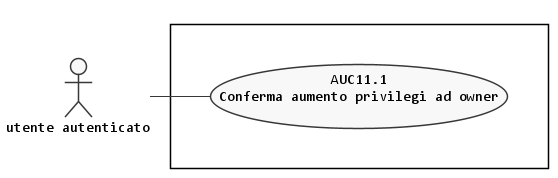
\includegraphics[width=100mm]{creazione-owner.png}
  \caption{AUC11: Creazione owner}%
  \label{fig:AUC11}
\end{figure}

\begin{description}
  \item[Codice:] AUC11;
  \item[Titolo:] Creazione owner;
  \item[Attori primari:] utente autenticato;
  \item[Precondizione:] il sistema deve rendere disponibile la pagina di creazione owner;
  \item[Postcondizione:] l'utente autenticato aumenta i suoi privilegi e diventa owner;
  \item[Scenario principale:]
  \begin{enumerate}
    \item un utente vuole diventare owner per poter creare una propria organizzazione.
  \end{enumerate}
\end{description}

\subsubsection{AUC11.1: Conferma aumento privilegi ad owner}%
\label{subs:AUC11.1}
\begin{description}
  \item[Codice:] AUC11.1;
  \item[Titolo:] Conferma aumento privilegi ad owner;
  \item[Attori primari:] utente autenticato;
  \item[Precondizione:] l'utente invia la richiesta di aumento privilegi;
  \item[Postcondizione:] l'utente autenticato aumenta i suoi privilegi e diventa owner;
  \item[Scenario principale:]
  \begin{enumerate}
    \item l'utente autenticato deve confermare l'aumento dei propri privilegi.
  \end{enumerate}
\end{description}

\end{document}
